\documentclass[12pt,fleqn,answers]{exam}
\usepackage{pifont}
\usepackage{dingbat}
\usepackage{amssymb}
\usepackage{epsfig}
\usepackage{graphicx}
\usepackage[]{hyperref}
\usepackage{geometry}
\usepackage[intlimits]{amsmath}
\geometry{letterpaper, margin=0.75in}
\addpoints
\boxedpoints
\pointsinmargin
\pointname{pts}

\usepackage[activate={true,nocompatibility},final,tracking=true,kerning=true,factor=1100,stretch=10,shrink=10]{microtype}
\usepackage[american]{babel}
%\usepackage[T1]{fontenc}
\usepackage{fourier}
\usepackage{isomath}
\usepackage{upgreek,amsmath}
\usepackage{amssymb}

\newcommand{\dotprod}{\, {\scriptzcriptztyle
    \stackrel{\bullet}{{}}}\,}

\newcommand{\reals}{\mathbf{R}}
\newcommand{\lub}{\mathrm{lub}} 
\newcommand{\glb}{\mathrm{glb}} 
\newcommand{\complex}{\mathbf{C}}
\newcommand{\dom}{\mbox{dom}}
\newcommand{\cover}{{\mathcal C}}
\newcommand{\integers}{\mathbf{Z}}
\newcommand{\vi}{\, \mathbf{i}}
\newcommand{\vj}{\, \mathbf{j}}
\newcommand{\vk}{\, \mathbf{k}}
\newcommand{\bi}{\, \mathbf{i}}
\newcommand{\bj}{\, \mathbf{j}}
\newcommand{\bk}{\, \mathbf{k}}
\DeclareMathOperator{\Arg}{\mathrm{Arg}}
\DeclareMathOperator{\Ln}{\mathrm{Ln}}
\newcommand{\imag}{\, \mathrm{i}}
\newcommand{\range}{\mathrm{range}}
\newcommand{\ball}{\mathrm{ball}}
\newcommand{\LP}{\mathrm{LP}}

\usepackage{graphicx}
\newcommand\AM{{\sc am}}
\newcommand\PM{{\sc pm}}
     
\newcommand{\quiz}{0}
\newcommand{\term}{Fall}
\newcommand{\due}{Friday 25 August  at 11:59 \PM}
\begin{document}
\large
\vspace{0.1in}
\noindent\makebox[3.0truein][l]{{\bf MATH 202}}
{\bf Name:} \hrulefill \\
\noindent \makebox[3.0truein][l]{\bf Calculus Practice III, \term \/ \the\year}
%{\bf Row:}\hrulefill\
\vspace{0.1in}

\noindent Here is an opportunity for you to maintain your calculus skills
over the summer. If you complete these problems,
digitize your work, and submit your work to Canvas, I will send you my
solutions. If you need some help with these questions, 
email me with your questions (\href{mailto:willisb@unk.edu}{willisb@unk.edu})

Completing this work is optional, and it does not 
enter into your class grade in any way--this work is 
 not a bonus, extra credit, or anything like that.

\begin{questions}


\question The graph in Figure 1 shows the graph of a wild and 
crazy function 
(the red curve) we'll unimaginatively call $F$. I've labeled 
 several points on the graph and I drew the tangent to the curve $y=F(x)$ with
the point of tangency $(x=2,y=5)$ as well.

\begin{parts}

\part As best you can, find the numerical value of $F^\prime(2)$. To do this, as accurately 
as your eyeballs allow, find the coordinates to two widely separated
points on tangent line (the green line) and find its slope using rise 
over run. 

\part For the other labeled points ($(-3,2),(-1,8)$, and $(1,8)$)
follow the same process to approximate the value of $F^\prime(-3),
F^\prime(-1)$ and $F^\prime(1)$. You'll need to use a ruler to 
draw each tangent line.

\part As best you can, draw a graph of $F^\prime$.
\end{parts}

\begin{figure}
\begin{center}
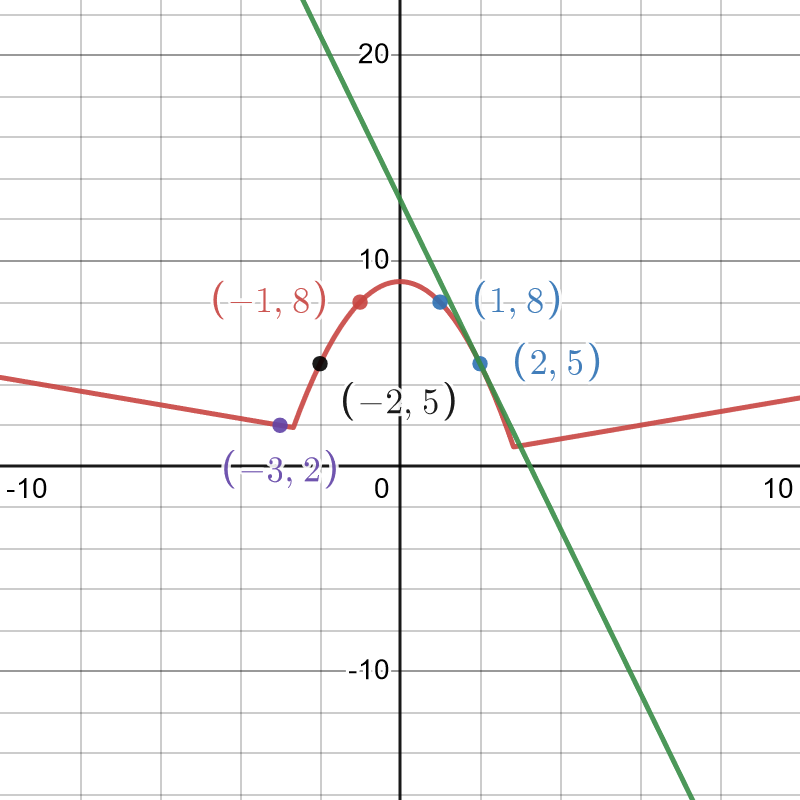
\includegraphics[scale=0.5]{desmos-graph(46).png}
\end{center}
\caption{Graph of some wild and crazy function (red curve) 
along with a graph of its tangent line at $(x=2,y=5).$}
\end{figure}
\end{questions}

%\max(-(x-3)/3,x/3,-(x^{2}-9))


\end{document}